\documentclass[a4paper, 11pt]{report}

\addtolength{\hoffset}{-1cm}
\addtolength{\textwidth}{2cm}

\usepackage[utf8]{inputenc}
\usepackage[frenchb]{babel}
\usepackage[T1]{fontenc}

\usepackage{graphicx}

\usepackage{hyperref}

%\usepackage{csquotes}

\usepackage{listings}
\usepackage{color}
\definecolor{lightgray}{rgb}{.9,.9,.9}
\definecolor{darkgray}{rgb}{.4,.4,.4}
\definecolor{purple}{rgb}{0.65, 0.12, 0.82}

\lstnewenvironment{OCaml}
                  {\lstset{
                      language=[Objective]Caml,
                      breaklines=true,
                      commentstyle=\color{purple},
                      stringstyle=\color{red},
                      identifierstyle=\ttfamily,
                      keywordstyle=\color{blue},
                      basicstyle=\footnotesize,
                      xleftmargin=0.15\textwidth
                    }
                  }
                  {}

\begin{document}

\chapter{Rapports de réunions de PSTL : \emph{interopérabilité entre OCaml et Java}}

Béatrice CARRE

Encadrants : Emmanuel Chailloux, Xavier Clerc, Grégoire Henry

\section*{Introduction}
Lien vers l'énnoncé du projet : 
\href{https://www-master.ufr-info-p6.jussieu.fr/2013/interoperabilite-entre-OCaml-et}{lien}.

\section{mardi 21 janvier : Le projet}
\subsection{sujets abordés}

Pour bien commencer, et établir un environnement de travail pratique
pour toute la durée du projet, l'élaboration d'un site de gestion de
version et un forum de conversation nous ont été fortement
recommandés.

Une fois ceci fait, nous aurons à installer et nous renseigner sur chacun des
outils que nous allons manipuler :
\begin{itemize}
\item Le projet OCaml-Java, un backend pour le compilateur binaire de Ocaml produisant du bytecode Java. \url{http://ocamljava.x9c.fr/preview/}
\item Le projet O'Jacaré, un générateur de code à partir d'un IDL, permettant l'interopérabilité entre OCaml et Java. \url{http://www.pps.univ-paris-diderot.fr/~henry/ojacare/}
\end{itemize}
Il nous a été conseillé de nous intéresser à différents documents
concernant O'Jacaré [1] et [2], et OCaml-Java [3] et [4].

\subsection{travail effectué}
Mise en place d'un forum de discussion :
\url{http://pstl-interop.forumserv.com}

Mise en place d'un site de gestion de version :
\url{https://github.com/beaCarre/PSTL}
\newline

L'installation d'O'Jacaré n'était pas possible, c'est pourquoi nous
nous sommes concentrés sur l'étude du projet OCaml-Java. 

Son code source n'étant pas accessible, nous avons étudié ses outils
et manuel utilisateur particulièrement bien détaillés sur le site. Les
exemples fournis nous ont beaucoup aidé à comprendre sa méthode, et à
maîtriser en partie son utilisation.

Nous avons surtout passé beaucoup de temps à lire des articles
(certains en anglais, donc beaucoup plsu de temps).
Mais ces articles, très intéressants, nous ont un peu ouvert les yeux sur
le sujet du projet et ont répondu à beaucoup de questions restées en
attente jusque là sur chacun des outils. 

\section{mercredi 12 février : Découverte d'OCaml Java}
\subsection{sujets abordés}
Nous avons fait un point sur la découverte d'Ocaml-Java. La question à
se poser est maintenant : comment modifier la génération d'O'Jacaré
pour obtenir les classes d'encapsulation adaptées pour OCaml-Java.
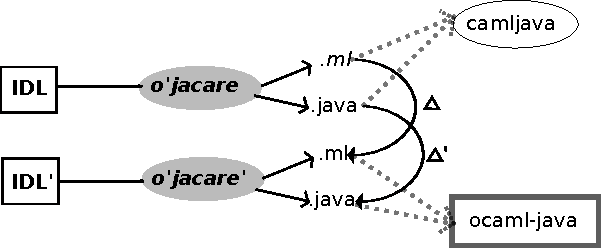
\includegraphics{schema1.pdf}
Dans le Schéma ci-dessus, montrant un schéma représentant le
méchanisme d'O'Jacaré.
L'intérêt est de connaître le \delta et
\delta'.
Plusieurs questions ou sujets ont été lancés :
\begin{itemize}
\item encapsulation des classes Java (wrapper) avec attribut callback
  TODO
\item voir héritage multiple O'Caml à partir de classes Java
  encapsulées TODO
\item le polymorphisme dans O'Jacaré TODO
\item l'intérêt d'un callback systématique (performances --)
\item faire peut-être dans un futur un paquet pour opam ?
\end{itemize}

Il existe un version d'O'Jacaré ayant été adaptées aux nouvelles
version d'OCaml, il nous est désormais accessible.
La seconde phase de ce projet sera d'explorer O'Jacaré, son code et
ses possibilités.
\subsection{travail effectué}
Nous avons commencé à développer des exemples pour explorer toutes ses
possibilités : un othello, en utilisant le OCaml pour le côté calcul,
et le Java et sa bibliothèque swing, pour le côté graphique. 

TODO : othello bloquée, à finir si c'ets possible

O'Jacaré a pu être installé et testé sur les exemples fournis.


TODO : finir othello pour O'Jacaré

\section{vendredi 21 février : Découverte d'O'Jacaré}
\subsection{sujets abordés}

schemas compil
\subsection{travail effectué}



\section{lundi 10 mars : Schémas de compilation d'O'Jacaré}
\subsection{sujets abordés}

\subsection{travail effectué (en conséquence ou non)}


\section*{References}
\begin{enumerate}
\item Cours 10 de MPIL : \emph{Interopérabilité OCaml et Java}, E. Chailloux,
\href{https://www-licence.ufr-info-p6.jussieu.fr/lmd/licence/2013/ue/LI332-2013oct/public/cours/COURS10.pdf}{lien}
\item \emph{O'Jacaré, une interface objet entre Objective Caml et Java}, E.Chailloux - G. Henry
\item\emph{OCaml-Java: Typing Java Accesses from OCaml Programs}, X. Clerc,
\href{http://www.cs.ru.nl/P.Achten/IFL2013/symposium_proceedings_IFL2013/ifl2013_submission_17.pdf}{lien}
\item \emph{OCaml-Java: from OCaml sources to Java bytecodes}, X. Clerc,
\href{http://www.lexifi.com/ml2012/full9.pd}{lien}
\item
\end{enumerate}
\end{document}
